%diplomovka
\documentclass[12pt, oneside]{book}
\usepackage[a4paper,top=2.5cm,bottom=2.5cm,left=3.5cm,right=2cm]{geometry}
\usepackage[utf8]{inputenc}
\usepackage[T1]{fontenc}
\usepackage{graphicx}
\usepackage{cite}
\usepackage{url}
\usepackage{amsthm}
\usepackage{amsmath}
\usepackage{mathrsfs}
\usepackage{amssymb}
\usepackage{enumitem}
\usepackage{tikz}
\usepackage{float}
\usepackage{verbatim}
\usetikzlibrary{automata,arrows,topaths}
\usepackage[slovak]{babel} % vypnite pre prace v anglictine
\linespread{1.25} % hodnota 1.25 by mala zodpovedat 1.5 riadkovaniu

\newtheorem{theorem}{Veta}[section]
\newtheorem{lemma}{Lema}[section]
\newtheorem{example}{Príklad}[section]
\newtheorem{definition}{Definícia}[section]
\newtheorem{notation}{Označenie}[section]
\newtheorem{note}{Poznámka}[section]
\newtheorem{corollary}{Dôsledok}[section]
\newtheorem{proposition}{Tvrdenie}[section]

% -------------------
% --- Definicia zakladnych pojmov
% --- Vyplnte podla vasho zadania
% -------------------
\def\mfrok{2017}
\def\mfnazov{Prídavná informácia a zložitosť nedeterministických konečných automatov}
\def\mftyp{Diplomová práca}
\def\mfautor{Bc. Šimon Sádovský}
\def\mfskolitel{prof. RNDr. Branislav Rovan, PhD.}

%ak mate konzultanta, odkomentujte aj jeho meno na titulnom liste
\def\mfkonzultant{tit. Meno Priezvisko, tit. }  

\def\mfmiesto{Bratislava, \mfrok}

%aj cislo odboru je povinne a je podla studijneho odboru autora prace
\def\mfodbor{2508 Informatika} 
\def\program{ Informatika }
\def\mfpracovisko{ Katedra informatiky }

\begin{document}     

% -------------------
% --- Obalka ------
% -------------------
\thispagestyle{empty}

\begin{center}
\sc\large
Univerzita Komenského v Bratislave\\
Fakulta matematiky, fyziky a informatiky

\vfill

{\LARGE\mfnazov}\\
\mftyp
\end{center}

\vfill

{\sc\large 
\noindent \mfrok\\
\mfautor
}

\eject % EOP i
% --- koniec obalky ----

% -------------------
% --- Titulný list
% -------------------

\thispagestyle{empty}
\noindent

\begin{center}
\sc  
\large
Univerzita Komenského v Bratislave\\
Fakulta matematiky, fyziky a informatiky

\vfill

{\LARGE\mfnazov}\\
\mftyp
\end{center}

\vfill

\noindent
\begin{tabular}{ll}
Študijný program: & \program \\
Študijný odbor: & \mfodbor \\
Školiace pracovisko: & \mfpracovisko \\
Školiteľ: & \mfskolitel \\
% Konzultant: & \mfkonzultant \\
\end{tabular}

\vfill


\noindent \mfmiesto\\
\mfautor

\eject % EOP i


% --- Koniec titulnej strany


% -------------------
% --- Zadanie z AIS
% -------------------
% v tlačenej verzii s podpismi zainteresovaných osôb.
% v elektronickej verzii sa zverejňuje zadanie bez podpisov

\newpage 
\thispagestyle{empty}
\hspace{-2cm}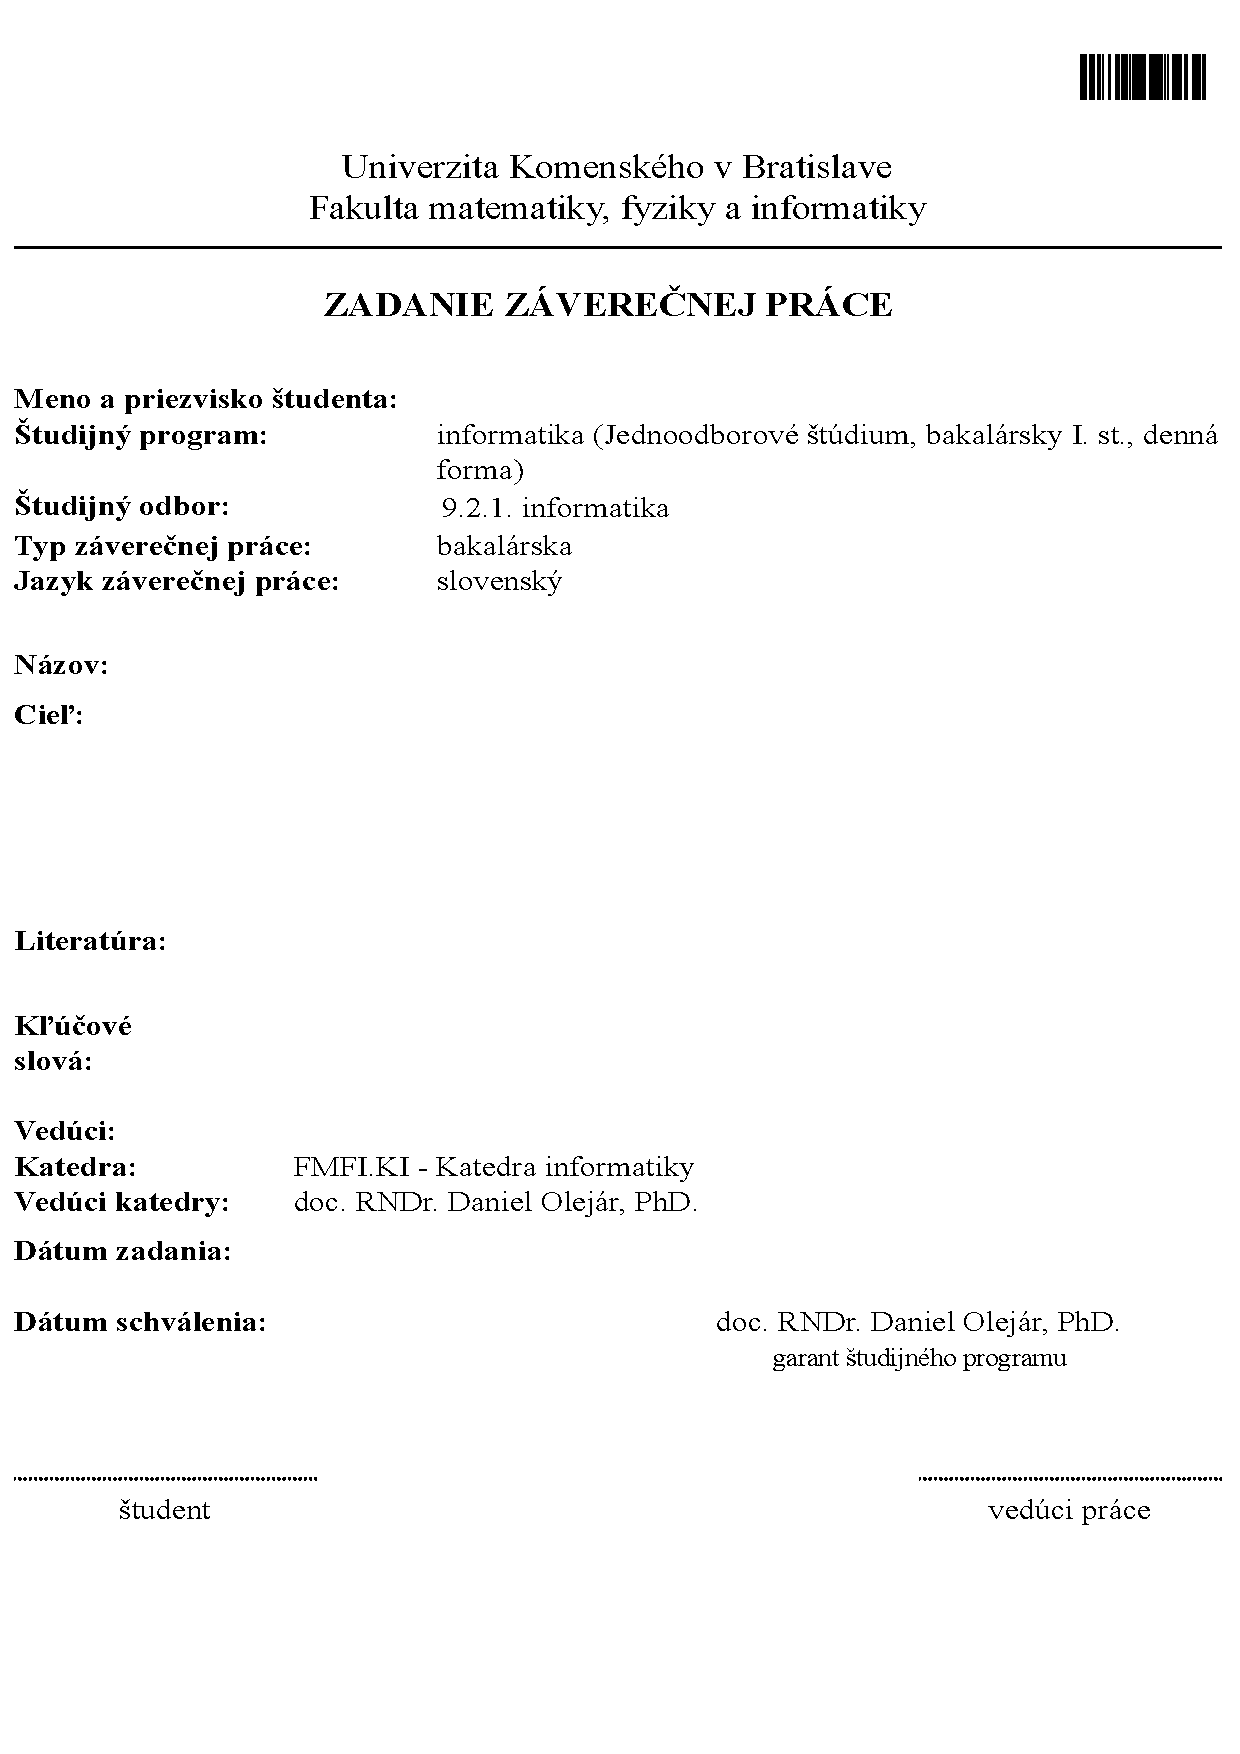
\includegraphics[width=1.1\textwidth]{images/zadanie}

% --- Koniec zadania

\frontmatter

% -------------------
%   Poďakovanie - nepovinné
% -------------------
\setcounter{page}{3}
\newpage 
~

\vfill
{\bf Poďakovanie:}

% --- Koniec poďakovania

% -------------------
%   Abstrakt - Slovensky
% -------------------
\newpage 
\section*{Abstrakt}

V práci skúmame vplyv prídavnej informácie na zložitosť riešenia problému. Ako výpočtový model sme zvolili nedeterministické konečné automaty a mierou zložitosti je počet stavov. Formalizáciou nášho problému je rozklad nedeterministického konečného automatu na dvojicu nedeterministických konečných automatov takých, že jazyk pôvodného automatu je prienikom jazykov týchto dvoch automatov. Navyše očakávame, že oba tieto automaty budú jednoduchšie ako pôvodný automat. V práci dokazujeme rozložiteľnosť respektíve nerozložiteľnosť konkrétnych regulárnych jazykov. Dokazujeme uzáverové a iné vlastnosti tried nedeterministicky rozložiteľných a nedeterministicky nerozložiteľných regulárnych jazykov. Charakterizujeme triedu jazykov tvorených jedným slovom vzhľadom na rozložiteľnosť. Skúmame jazyky, ktorých minimálny nedeterministický automat je tvorený práve jedným cyklom. Ukazujeme rozdiel medzi nedeterministickou a deterministickou rozložiteľnosťou regulárnych jazykov.

\paragraph*{Kľúčové slová:} nedeterministický konečný automat, rozklad nedeterministického konečného automatu, nedeterministická rozložiteľnosť, prídavná informácia, popisná zložitosť
% --- Koniec Abstrakt - Slovensky


% -------------------
% --- Abstrakt - Anglicky 
% -------------------
\newpage 
\section*{Abstract}

We study the effect of supplementary information on the complexity of problem solution. We have chosen nondeterministic finite automaton as the computational model and we measure the complexity by the number of states. We formalize our problem via decomposition of nondeterministic finite automaton into two nondeterministic finite automata, such that the language accepted by the original automaton is the intersection of languages accepted by this two automata. Moreover, we require both automata in the decomposition to be simpler than the original automaton. We show decomposability and nondecomposability of particular regular languages. We show closure and other properties of classes of nondeterministically decomposable and nondecomposable regular languages. We characterize the class of languages consisting of exactly one word with respect to decomposability. We examine languages accepted by nondeterministic automata consisting of exactly one cycle. We show the difference between nondeterministic and deterministic decomposability of regular languages.


\paragraph*{Keywords:} nondeterministic finite automaton, decomposition of nondeterministic finite automaton, nondeterministic decomposability, supplementary information, descriptional complexity

% --- Koniec Abstrakt - Anglicky

% -------------------
% --- Predhovor - v informatike sa zvacsa nepouziva
% -------------------
%\newpage 
%\thispagestyle{empty}
%
%\huge{Predhovor}
%\normalsize
%\newline
%Predhovor je všeobecná informácia o práci, obsahuje hlavnú charakteristiku práce 
%a okolnosti jej vzniku. Autor zdôvodní výber témy, stručne informuje o cieľoch 
%a význame práce, spomenie domáci a zahraničný kontext, komu je práca určená, 
%použité metódy, stav poznania; autor stručne charakterizuje svoj prístup a svoje 
%hľadisko. 
%
% --- Koniec Predhovor


% -------------------
% --- Obsah
% -------------------

\newpage 

\tableofcontents

% ---  Koniec Obsahu

% -------------------
% --- Zoznamy tabuliek, obrázkov - nepovinne
% -------------------

\newpage 

\listoffigures

% ---  Koniec Zoznamov

\mainmatter


\input uvod.tex

\input definicie.tex

\input rozlozitelneNerozlozitelne.tex

\input detVsNdet.tex

\input vlastnostiRNR.tex

\input zaver.tex

% -------------------
% --- Bibliografia
% -------------------


\newpage	

\backmatter

\thispagestyle{empty}
\nocite{*}
\clearpage

\bibliographystyle{apalike}
\bibliography{literatura}

%Prípadne môžete napísať literatúru priamo tu
%\begin{thebibliography}{5}
 
%\bibitem{br1} MOLINA H. G. - ULLMAN J. D. - WIDOM J., 2002, Database Systems, Upper Saddle River : Prentice-Hall, 2002, 1119 s., Pearson International edition, 0-13-098043-9

%\bibitem{br2} MOLINA H. G. - ULLMAN J. D. - WIDOM J., 2000 , Databasse System implementation, New Jersey : Prentice-Hall, 2000, 653s., ???

%\bibitem{br3} ULLMAN J. D. - WIDOM J., 1997, A First Course in Database Systems, New Jersey : Prentice-Hall, 1997, 470s., 

%\bibitem{br4} PREFUSE, 2007, The Prefuse visualization toolkit,  [online] Dostupné na internete: <http://prefuse.org/>

%\bibitem{br5} PREFUSE Forum, Sourceforge - Prefuse Forum,  [online] Dostupné na internete: <http://sourceforge.net/projects/prefuse/>

%\end{thebibliography}

%---koniec Referencii

% -------------------
%--- Prilohy---
% -------------------

%Nepovinná časť prílohy obsahuje materiály, ktoré neboli zaradené priamo  do textu. Každá príloha sa začína na novej strane.
%Zoznam príloh je súčasťou obsahu.
%
%\addcontentsline{toc}{chapter}{Appendix A}
%\input AppendixA.tex
%
%\addcontentsline{toc}{chapter}{Appendix B}
%\input AppendixB.tex

\end{document}






